\documentclass[10pt,a4paper]{article}
\usepackage[a4paper,margin=2.1cm,top=2.4cm,bottom=2.3cm]{geometry}
\usepackage[T1]{fontenc}
\usepackage[utf8]{inputenc}
\usepackage{helvet}
\renewcommand{\familydefault}{\sfdefault}
\usepackage{amsmath,amssymb}
\usepackage{xcolor}
\usepackage{graphicx}
\graphicspath{{figures/}{logos/}}
\usepackage{booktabs,tabularx,longtable,multirow}
\usepackage{enumitem}
\usepackage{titlesec}
\usepackage{fancyhdr}
\usepackage{caption}
\usepackage{url}
\usepackage{tcolorbox}\tcbuselibrary{breakable}
\usepackage[colorlinks=true,linkcolor=cernblue,urlcolor=cernblue,citecolor=cernblue]{hyperref}

\definecolor{cernblue}{HTML}{0053A1}
\definecolor{shorange}{HTML}{D55E00}
\definecolor{okgreen}{HTML}{1B7F3B}
\definecolor{greytxt}{HTML}{555555}
\definecolor{lightblue}{HTML}{EAF1F9}

\setlist{itemsep=1pt,topsep=2pt,leftmargin=1.4em}
\titleformat{\section}{\Large\bfseries\color{cernblue}}{\thesection}{0.6em}{}
\titleformat{\subsection}{\large\bfseries\color{cernblue}}{\thesubsection}{0.6em}{}
\titlespacing*{\section}{0pt}{14pt}{6pt}
\captionsetup{font=small,labelfont={bf,color=cernblue}}

\pagestyle{fancy}
\fancyhf{}
\renewcommand{\headrulewidth}{0pt}
\fancyfoot[L]{\color{greytxt}\footnotesize SHiP veto background study --- status on 10 November 2026}
\fancyfoot[R]{\color{greytxt}\footnotesize \thepage}

% tags
\newcommand{\solid}{\textcolor{okgreen}{\textbf{solid}}}
\newcommand{\est}{\textcolor{shorange}{\textbf{estimate}}}
\newcommand{\open}{\textcolor{shorange}{\textbf{open}}}
\newcommand{\src}[1]{{\color{greytxt}\footnotesize[\texttt{\detokenize{#1}}]}}
\newcommand{\note}[1]{\begin{tcolorbox}[colback=lightblue,colframe=lightblue,arc=1mm,left=6pt,right=6pt,top=3pt,bottom=3pt]\small #1\end{tcolorbox}}
\newcommand{\pot}{p.o.t.}

\begin{document}
\sloppy

\thispagestyle{fancy}
\begin{tcolorbox}[colback=cernblue,colframe=cernblue,arc=0mm,left=10pt,right=10pt,top=8pt,bottom=8pt]
\color{white}
\begin{minipage}[c]{0.74\linewidth}
{\LARGE\bfseries Veto system background study}\\[3pt]
{\Large Status quo}\\[6pt]
{\normalsize \underline{G.~Frisella}$^{1,2}$, S.~R.~Qasim$^{1}$ \quad 10 November 2026}
\end{minipage}\hfill
\begin{minipage}[c]{0.24\linewidth}\raggedleft

\includegraphics[height=1.25cm]{ship-logo-white.png}\\[4pt]

\includegraphics[height=0.75cm]{uzh-logo-white.png}
\end{minipage}
\end{tcolorbox}
{\footnotesize\color{greytxt}$^1$ University of Zurich, $^2$ European Organization for Nuclear Research (CERN)}

\medskip
\noindent This note gives the state of the background estimate for the SHiP decay-vessel veto after PR~\#15
(merged 10 Nov 2026) and the V0-production check of the same day. Every number points to the file it comes from
(\src{...}, paths relative to \path{Optimization_Veto_System/veto/}). Rates are per spill of $4\times10^{13}$\,\pot{}
(= kHz at $4\times10^{13}$\,\pot/s); yields are per 15 years ($6\times10^{20}$\,\pot{} = $1.5\times10^{7}$ spills).
Reference design: \texttt{D6\_straw\_mod}. Each result is tagged \solid{} (checked by an independent method),
\est{} (extrapolated or model-dependent) or \open{} (known disagreement, not resolved).

\section{Executive summary}

\begin{table}[h]
\centering\small
\caption{Background budget for \texttt{D6\_straw\_mod}, per 15 years, after the full selection and the veto
(level b = reconstructed veto; level c = truth). ``Straight'' = products as straight lines after the source,
``G4'' = products through Geant4 (\texttt{g4vessel}) downstream.}
\label{tab:budget}
\begin{tabularx}{\linewidth}{@{}l r X l@{}}
\toprule
Source & after veto / 15\,y & Comment & Tag\\
\midrule
MS7 muon DIS $\to K_L$ (last 50\,cm of iron) & $\sim1.5\times10^{4}$ & range $1$--$2\times10^4$ from the IP$^2$ extrapolation; direct re-decay count $1.39\times10^4$ selected, $9.7\times10^3$ after veto (13 MC events). Not vetoable (decay tracks have no upstream hits). FairShip sees none (D3). & \est, \open\\
Muon DIS in the helium & 472 & 1.82e3 selected; 673 at truth level c (parent crossed no plane: side-entry coverage gap). & \est\\
Muon DIS in the vessel walls & 44 & 176 selected. & \est\\
Neutrino DIS in the vessel (He + walls) & 1.5 & 1.3 He + 0.2 walls (G4); 3.0--3.3 with straight lines. & \solid\\
Neutrino DIS in MS7 & 1.0 & 2.2--2.4 with straight lines. & \solid\\
Muon combinatorial ($\mu\times\mu$) & 0.014 & Nov-4 inputs (0.003 with EM debris); dataset c gives 51: source-tail question open. & \open\\
$\mu\times$rock tracks & 0.023 & rock leg vetoed 99.99\,\%. & \est\\
Muon / neutrino DIS in the cavern rock & 0 & 0 selected; muon rock bounded statistically only at $<1.6\times10^8$, the zero rests on geometry (IP $\ge 12.6$\,m). & \est\\
\midrule
EM debris (shield end) & -- & enters as accidental hits: signal loss $6.4\,\% \to 7.5\,\%$. & \est\\
\bottomrule
\end{tabularx}\\[2pt]
{\footnotesize Sources: \path{docs/STATUS.md} (sections 2026-11-09 evening, 2026-11-10 event store, night runs),
\path{docs/neutrinos_2026.md}, \path{ISSUES.txt} D2, D3, D7, D14.}
\end{table}

\paragraph{Messages.}
\begin{enumerate}
\item \textbf{The MS7 $K_L$ dominates by $\times30$} over the next source. Production in the iron is validated by
natural Geant4 (Sec.~\ref{sec:ms7}) and the $K^0_S$/$\Lambda$ yields of the Geant4 generator agree with
$\gamma p$ data at $W\simeq6$\,GeV within $\sim6\,\%$, while Pythia~6 is $\times1.9$ high. What is \emph{not}
understood is why FairShip sees zero MS7 $K^0$-decay tracks where the chain expects 7.9 entries ($P=4\times10^{-4}$).
The number rests on 13 MC events after the selection: a $K_L$-enriched generation is needed.
\item \textbf{Muon DIS in the helium is not small} (correction of 10 Nov): 472 after the veto, a side-entry coverage
gap of the straw design.
\item \textbf{Neutrinos} with the 2026 flux and GENIE v2: $\sim2.5$ per 15\,y in total (vessel 1.5 + MS7 1.0, Geant4
downstream), irreducible for an upstream veto; a lateral-track veto could remove up to 77\,\% of the helium ones (D2).
\item \textbf{Combinatorial} pairs: 0.014 on the Nov-4 inputs vs 51 on dataset c for the same design. Explained by a
$\times3$--4 harder near-axis source tail in dataset c (rate $\propto$ square); which tail is right is open (D5).
\item \textbf{Cavern rock} adds 8$\times$ the combinatorial candidates but nothing after the veto.
\end{enumerate}

\note{\textbf{What is solid:} neutrino flux (validated vs GSimple 2026 and SHiP 2025 SND rates), K$_L$ production in the
MS7 iron (natural Geant4), V0 multiplicities vs data at $W\simeq6$\,GeV, forced-decay tables (PDG).
\textbf{What is not:} the FairShip MS7 gap (D3), the muon source tail (D5, enters the combinatorial as a square),
the 13-MC-event MS7 selected number, the helium coverage gap, the rock zero (geometric argument).}

\section{Setup and conventions}

\begin{itemize}
\item \textbf{Layout} (since 5 Nov 2026): FairShip \texttt{geometry\_config.py} 2026-0.1 in the target-aligned frame
$z_\text{veto}=z_\text{FS}-2.14$\,m: shield end 29.89\,m, vessel 31.13--81.13\,m (UBT on the entrance window),
straw stations 82.08 / 84.08 / 91.08 / 93.08\,m, timing detector 94.01\,m ($5.5\times6.5$\,m), spectrometer magnet
84.36--89.56\,m. Stored muon states stay at 30.6 / 82.0\,m; every crossing is computed from them. Results older than
5 Nov use the old layout. \src{ISSUES.txt GEOMETRY}
\item \textbf{Normalisation}: $4\times10^{13}$\,\pot{} per spill everywhere (D13, legacy inputs rescaled when read),
15\,y = $1.5\times10^7$ spills. Flat 1\,s spill (A5).
\item \textbf{Muon source}: \texttt{target-production-complete-november-4-2026} (FairShip target, Pythia 8.223,
Geant4 11.2 FTFP\_BERT, every muon source forced and weighted, 10\,GeV threshold), validated against unforced
production (27 species within $2\sigma$, full events $1.003\pm0.005$) and reproducing the 2018 FairShip files to
1--3\,\% once FairShip's 2018 weighting is applied (Fig.~\ref{fig:source}). The 2018 files lack $\sim22$--24\,\% of the
physical flux ($\eta\to\mu\mu\gamma$, $\omega\to\pi^0\mu\mu$). \src{docs/STATUS.md (1 Nov, 4 Nov)}
\item \textbf{Muon flow per spill}: $4.69\times10^{10}$ from the target, $4.38\times10^{10}$ stop in the shield,
$3.11\times10^{9}$ reach 30.6\,m ($1.46\times10^9$ into the $-x$ wall, $9.1\times10^7$ into the floor),
$\sim3\times10^{4}$ reach SST1. \src{docs/STATUS.md (2026-11-08)}
\item \textbf{Transport}: cuda-muons (TRY6 shield, field, rock), shell storage around the vessel (3\,780 seeds).
\item \textbf{MS7 chain default}: Geant4 11.2 muonNuclear (D3 decision of 9 Nov); Pythia 6 / Pythia 8 as the generator
systematic.
\item \textbf{Selection}: $\ge2$ good tracks at SST1, fiducial, measured IP $<10$\,cm (fully reconstructed) or
$<2.5$\,m (partially reconstructed); veto levels b (reconstructed hits) and c (truth).
\end{itemize}

\begin{figure}[h]
\centering
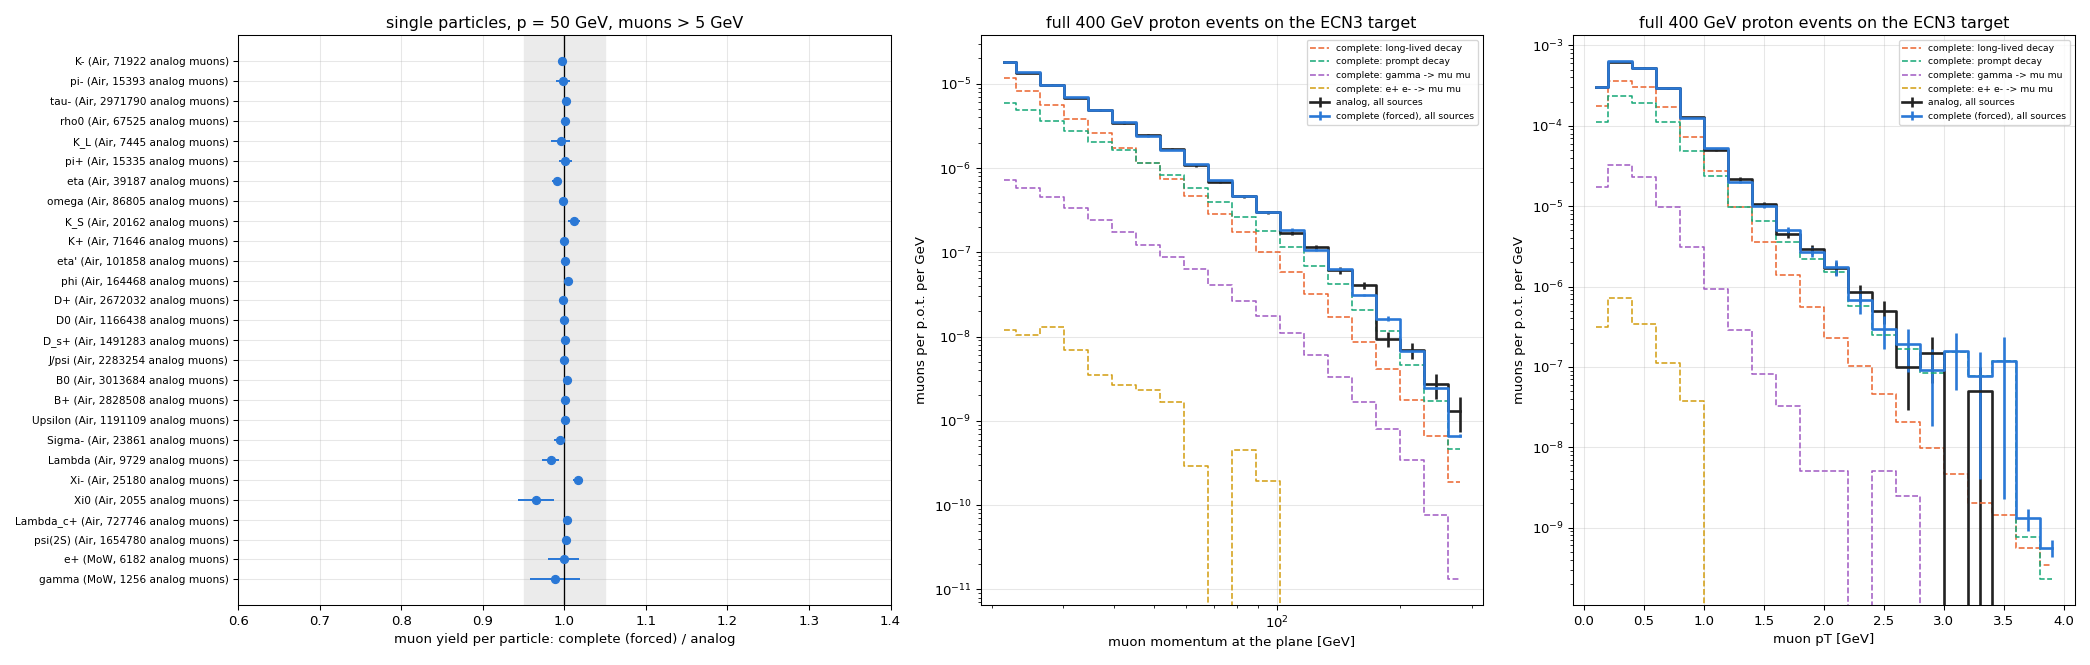
\includegraphics[width=\linewidth]{complete_validation.png}
\caption{Validation of the complete target production (forced vs analog, per species and full events).
\src{lhcb_data .../results/complete_validation/complete_validation.png}}
\label{fig:source}
\end{figure}

\section{Muon combinatorial background}

Two unrelated muons in time that form a vertex pointing to the target.

\begin{table}[h]
\centering\small
\caption{\texttt{D6\_straw\_mod}, per 15 years. \src{docs/STATUS.md (2026-11-09, 2026-11-10 night)}}
\begin{tabular}{@{}lrrrl@{}}
\toprule
Inputs & candidates & IP $<10$\,cm & after veto & note\\
\midrule
dataset c (\texttt{inputs\_c\_s}), $\mu\times\mu$ & 852 & 405 & 51 & legs explained 0.74 / 0.64\\
dataset c, $\mu\times$rock & 8\,190 & 2\,927 & 0.023 & rock leg explained 0.9999\\
dataset c, rock$\times$rock & $5\times10^{-7}$ & 0 & 0 & \\
Nov-4 (\texttt{inputs\_nov4}), $\mu\times\mu$ & 2.86 & -- & 0.014 & 0.003 with EM debris\\
\bottomrule
\end{tabular}
\end{table}

\begin{itemize}
\item The $\times140$ difference between dataset c and Nov-4 is \textbf{not the layout}: dataset c has 3--4$\times$ more
SST1 muons at 30--100\,GeV near the axis (source pool, D5), the pair rate goes as the square, times the pointing
preference, times the old $5\times10^{13}$ normalisation of \texttt{inputs\_c\_s}. \open: compare pool v2/v3 and Nov-4
spectra above 100\,GeV by component.
\item On the factorised estimate (A1): closure on \texttt{inputs.npz} D0\_minimal 1\,694 observed vs 1\,702 factorised
($p=0.86$); for vetoed designs 0 observed, $<7.6\times10^{-4}$ (90\,\% CL). \src{ISSUES.txt A1}
\item Source systematic (D5): the enriched tail's angles raise the SST1-selected rate by $\times1.55$ (convention
$\times0.905$, tail angles $\times0.56$); kept as is, quoted as $+40\,\%$ on the SST1-selected rate.
\end{itemize}

\begin{figure}[h]
\centering
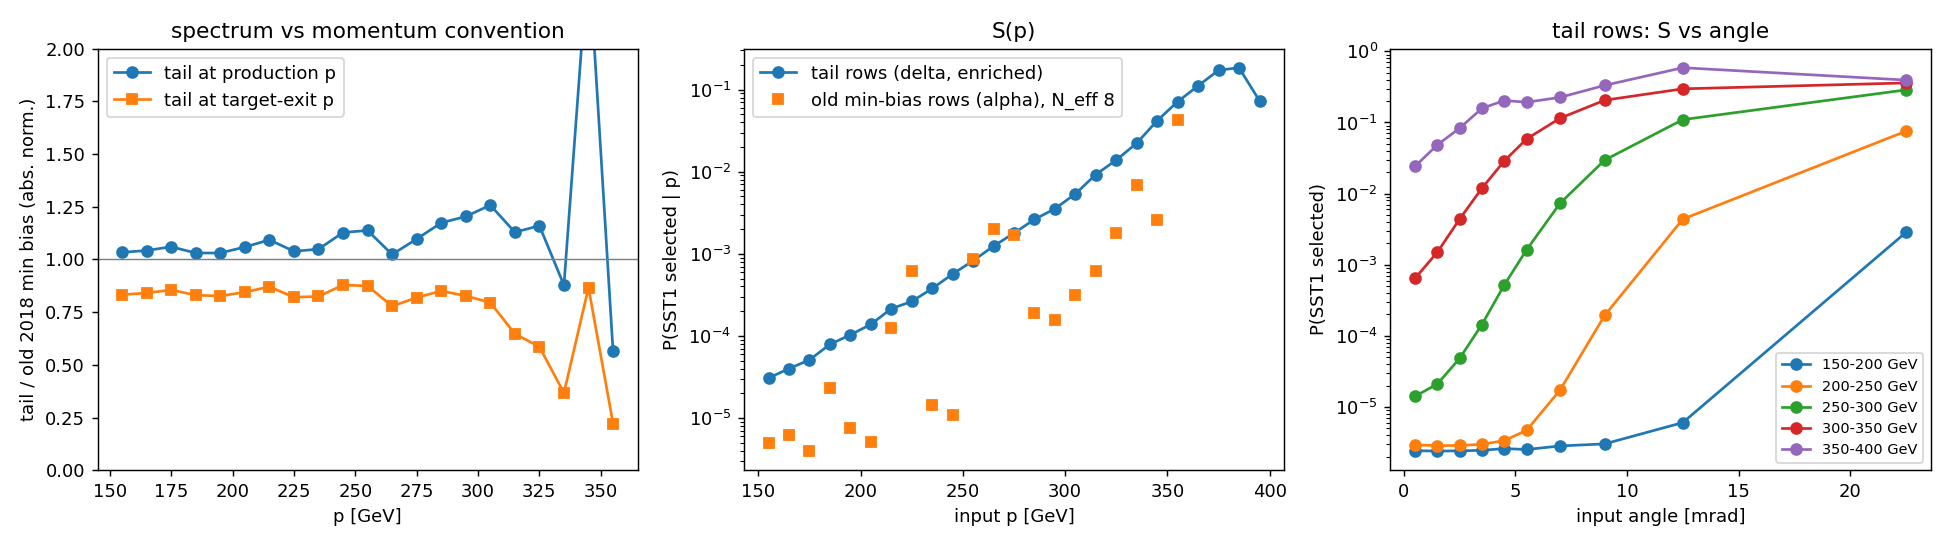
\includegraphics[width=0.95\linewidth]{d5_summary.png}
\caption{D5 check: momentum convention and tail angles of the enriched source. \src{results/d5_convention/d5_summary.png}}
\end{figure}

\section{Muon DIS in the vessel: helium, walls, planes, air}

Forced muon interactions along the stored trajectories (fastveto library: Geant4 muonNuclear at low $\nu$,
Pythia~6 above), products optionally through Geant4 in the vessel.

\begin{table}[h]
\centering\small
\caption{\texttt{D6\_straw\_mod} on the Nov-4 muons (\texttt{run\_interactions --kind muon}), per 15 years.
\src{docs/STATUS.md (2026-11-10 night, ``Correction'')}}
\begin{tabular}{@{}lrrr@{}}
\toprule
Target & selected & after veto b & truth level c\\
\midrule
helium & 1\,820 & 472 & 673\\
vessel walls (Mylar) & 176 & 44 & --\\
\bottomrule
\end{tabular}
\end{table}

\begin{itemize}
\item \textbf{Correction (10 Nov)}: the helium DIS was believed small; it is the \textbf{second background after the
MS7 $K_L$}. At truth level the parent crossed no veto plane: muons entering through the side are a coverage gap of
this straw design. For comparison, dataset c gave 210--250 for D6\_tile2 / E3 / E4 / E5 (e2e\_c). Store:
\path{vessel_mu_nov4_D6_straw_mod} ($7.0\times10^6$ events). \est
\item Air near the vessel and fins: done (C7, 5 Nov); old PVC wall results to be redone with Mylar (D8, \open).
\item Statistics: helium sufficient now ($\times20$ later), walls lacking (22 per MC event, cheap to improve).
\end{itemize}

\clearpage
\section{MS7 shield DIS $\to$ V0 decaying in the vessel}
\label{sec:ms7}

\subsection{Chain}
Parents: muons crossing the last 50\,cm of MS7 iron ($z=29.39$--29.89\,m, $|x|<1.71$, $|y|<1.27$\,m), bent by the
field; forced muon-nuclear interaction uniform along the chord; final state from the iron library; Geant4 (FTFP\_BERT,
MS7 field) to the exit plane $z=29.90$\,m; every $K_L$, $K_S$, $\Lambda$, $\Xi^0$ there forced to decay in the vessel
(Fig.~\ref{fig:chain}). \src{bin/shield_dis.py, docs/shield_iron_dis.md}

\begin{figure}[h]
\centering
\includegraphics[height=8.5cm]{dis_chain_overview.pdf}\hfill
\includegraphics[width=0.52\linewidth]{dis_sigma_generators.pdf}
\caption{Left: the forced chain. Right: muon-nuclear cross section per nucleon in iron for the generators (Geant4
muonNuclear includes the soft photonuclear part; Pythia only the DIS part).
\src{docs/dis_chain_pdf/overview.pdf, results/shield_dis/dis_sigma_generators.pdf}}
\label{fig:chain}
\end{figure}

\subsection{Rates (PR \#15, Geant4 11.2, 10 runs $\times\,2\times10^6$ interactions)}
\begin{itemize}
\item $7.94\times10^{5}$ interactions per spill ($1.19\times10^{13}$ per 15\,y); at the exit plane ($p>1$\,GeV):
$K_L$ 2\,923, $K_S$ 473, $\Lambda$ 262 per spill. \src{results/shield_dis/shield_muon_g4v112_s1??.json}
\item V0 decays in the vessel: 1\,547 per spill ($K_L$ 1\,540) $=2.33\times10^{10}$ per 15\,y; on the Nov-4 parents
$2.69\times10^{10}$ (parents $\times1.19$).
\item Selection: 0 selected in each file. All cuts but IP: $1.4\times10^7$; IP $<2/1/0.5/0.25/0.1$\,m:
$8.1\times10^6$ / $2.1\times10^6$ / $3.8\times10^5$ / $7.6\times10^4$ / $1.8\times10^4$ ($356/98/18/3/1$ MC). Near 0 the
tail goes as IP$^2$ $\Rightarrow$ \textbf{$\sim1.5\times10^4$ per 15\,y} (range 1--2$\times10^4$), confirmed by 100
re-decays of the 14\,168 pre-selected V0: $1.39\times10^4$ selected (13 MC), $9.7\times10^3$ after veto. \est
\item With Geant4 downstream (g4vessel): all-but-IP $1.44\times10^7$ (straight $1.95\times10^7$), IP $<1$\,m
$2.0\times10^6$.
\end{itemize}

\subsection{Validation and the FairShip disagreement (D3)}
\begin{table}[h]
\centering\small
\caption{Leaving the iron, $p>1$\,GeV, per spill: natural Geant4 10.7.3 (no forcing) vs the forced chain.
\src{docs/shield_iron_dis.md (natural Geant4)}}
\begin{tabular}{@{}lrrr@{}}
\toprule
 & natural, QGSP\_BERT\_HP\_PEN & natural, FTFP\_BERT & chain, G4 10.7 (forced)\\
\midrule
$K_L$ & $3\,499\pm128$ & $3\,686\pm130$ & 3\,387\\
$\pi^\pm$ & 93\,770 & 92\,970 & 93\,090\\
$K^\pm$ & 7\,014 & 7\,108 & 6\,704\\
$K_S$ / $\Lambda$ & 1\,728 / 907 & 1\,522 / 915 & 582 / 286\\
\bottomrule
\end{tabular}
\end{table}
\begin{itemize}
\item The chain reproduces natural Geant4 for $K_L$, $\pi$, $K^\pm$, $p$, $n$ \solid; $K_S$/$\Lambda$ are $3\times$ low
because the default library decays them at the vertex (D9).
\item Generators: $K_L$ decays in the vessel per spill Pythia~6 5\,604, crossover 5\,170, Geant4 11.2 2\,140, Geant4
10.7 2\,260 (6 Nov runs, earlier parents). 98\,\% of the Geant4 $K_L$ come from $Q^2<1$\,GeV$^2$, 55\,\% from
$W=5$--10\,GeV (Fig.~\ref{fig:q2w}). Hard part only ($Q^2>1$): Pythia~8 gives $\div6$ fewer $K_L$ than Pythia~6.
\item \open{} FairShip full simulation (\texttt{TRY\_2026\_EM\_SST1\_origin}) has 0 MS7 $K^0$-decay tracks; with the
tracking cuts the chain expects 7.9 entries ($P(0)=4\times10^{-4}$). Not the generator, not the physics list, not the
muon-nuclear definition. Left: the parent flux into MS7 (TRY6 vs TRY\_2026), FairShip event filtering / weights, the
$K_L$ handling downstream. Next: small FairShip run with our MS7 parents.
\end{itemize}

\begin{figure}[h]
\centering
\includegraphics[width=0.55\linewidth]{kl_q2w_A_geant4_11.2.pdf}
\caption{$Q^2$ and $W$ of the interactions that make the $K_L$ (Geant4 11.2, generator level).
\src{results/shield_dis/kl_q2w_A_geant4_11.2.pdf}}
\label{fig:q2w}
\end{figure}

\subsection{V0 production compared with data (D16, 10 Nov)}
Every V0 made at the vertex, also those absorbed or decayed in the iron: V0-stable library (same Geant4 11.2 model,
$K_S$/$\Lambda$ undecayed) folded with the vertex-energy spectrum of the PR runs (median 72\,GeV).
\src{bin/v0_production.py, docs/v0_production.md}

\begin{figure}[h]
\centering
\includegraphics[width=\linewidth]{v0_vs_W.pdf}
\caption{Left: mean V0 multiplicity per interaction vs $W$, Geant4 (solid) and Pythia~6 (dashed); stars:
$\gamma p$ at $E_\gamma=20$\,GeV \cite{abe1984}. Right: $W$ of the library events (Geant4 median 1.3\,GeV, below the
$K\Lambda$ threshold).}
\label{fig:v0w}
\end{figure}

\begin{table}[h]
\centering\small
\caption{Per event at $W=6.2\pm0.5$\,GeV. Data on hydrogen, Geant4 on Fe, Pythia~6 on free $p$/$n$.}
\begin{tabular}{@{}lrrr@{}}
\toprule
 & $K^0_S$ & $\Lambda$ (+$\Sigma^0$) & $\bar\Lambda$\\
\midrule
$\gamma p$, $E_\gamma=20$\,GeV, SLAC SHF \cite{abe1984} & $0.082\pm0.003$ & $0.049\pm0.002$ & $0.0029\pm0.0003$\\
Geant4 11.2 muonNuclear (8\,381 ev) & 0.087 & 0.051 & 0.0020\\
Pythia 6 ($1.2\times10^5$ ev) & 0.153 & 0.090 & 0.0058\\
\midrule
\multicolumn{4}{@{}l}{\footnotesize reference, not $W$-matched: NOMAD $\nu_\mu$ CC on C, $\langle E_\nu\rangle=45$\,GeV
\cite{nomad2002}: 0.0676 / 0.0504 / 0.0037}\\
\bottomrule
\end{tabular}
\end{table}

\begin{itemize}
\item Geant4 agrees with the data within $\sim6\,\%$ \solid; Pythia~6 is $\times1.9$ high: data support Geant4 as the
default, and the Pythia $\times2.7$ spread is one-sided. The low-$W$ region (1.6--3\,GeV), where most Geant4 events are,
is not yet compared (\open: CLAS / SAPHIR exclusive data).
\item Made per spill: $K_L$ $7.9\times10^3$, $K_S$ $7.8\times10^3$, $\Lambda$ $5.4\times10^3$, $\bar\Lambda$ 260
($K_L=K_S$ as required); per 15\,y $1.2\times10^{11}$ $K_L$. V0 are soft (median $p$ 1.4--2.5\,GeV).
\item $K_L$ budget per spill: $7.9\times10^3$ made $\to$ $6.5\times10^3$ with $T>0.5$\,GeV (plane cut) $\to$
2.0--2.5$\times10^3$ survive the iron ($\lambda=17$--22\,cm) $\to$ $3.1\times10^3$ at the exit (21--37\,\% made by the
shower in the iron, \est) $\to$ 1\,540 decay in the vessel ($P=0.49$, PDG $c\tau$).
\item $K_S$/$\Lambda$ at the exit rise with vertex depth up to $\sim12$\,cm: shower build-up (Fig.~\ref{fig:fate}).
\item Decay tables vs PDG: $c\tau$ and branching ratios correct; $K_L\to\pi^+\pi^-$ ($2\times10^{-3}$, a 2-track vertex
pointing to the shield, $\sim5\times10^7$ in the vessel per 15\,y) and $K_L\to\gamma\gamma$ missing.
\end{itemize}

\begin{figure}[h]
\centering
\includegraphics[width=\linewidth]{v0_ms7_fate.pdf}
\caption{Left: V0 per interaction vs muon energy (grey: MS7 interaction spectrum). Right: V0 at the exit plane per
interaction vs vertex depth; dotted / dash-dotted: primary $K_L$ only.}
\label{fig:fate}
\end{figure}

\section{Neutrinos}

\paragraph{Flux.} New production with the 2026 target (\texttt{nu\_prod.sbatch}): per proton $\nu_\mu$
$5.50\times10^{-3}$ ($2.2\times10^{11}$/spill), $\bar\nu_\mu$ $3.94\times10^{-3}$, $\nu_e$ $5.55\times10^{-4}$ (46\,\%
charm), $\bar\nu_e$ $5.29\times10^{-4}$, $\nu_\tau$/$\bar\nu_\tau$ $3.9\times10^{-5}$ each. Validated \solid: $\nu_\mu$
within 1--4\,\% of the GSimple 2026 flux; folded on a 3\,t W block it gives the SHiP 2025 SND CC rates
\cite{ship2025} within 20--30\,\% per flavour. The 2018 flux was $\times2$--2.7 low ($\nu$ kept only with a stored
sister muon $>15$\,GeV, no $E<10$\,GeV, no $\nu_e$/$\nu_\tau$). \src{docs/neutrinos_2026.md}

\paragraph{Interactions.} GENIE 3.06.02 library v2 (6 flavours $\times$ 15 nuclei incl.\ Fe56 and concrete).

\begin{table}[h]
\centering\small
\caption{\texttt{D6\_straw\_mod}, per 15 years. Straight lines after the vertex vs Geant4 downstream.
\src{docs/neutrinos_2026.md, docs/STATUS.md (2026-11-10 night)}}
\begin{tabular}{@{}lrrrr@{}}
\toprule
 & interactions & selected & after veto b (straight) & after veto b (G4)\\
\midrule
$\nu_\mu$ & $8.5\times10^4$ & 1.25 & 1.02 & 0.42 + 0.06\\
$\bar\nu_\mu$ & $3.2\times10^4$ & 0.57 & 0.51 & 0.16 + 0.10\\
$\nu_e$ & $2.6\times10^4$ & 1.57 & 1.37 & 0.59 + 0.02\\
$\bar\nu_e$ & $1.2\times10^4$ & 0.43 & 0.39 & 0.15 + 0.03\\
$\nu_\tau+\bar\nu_\tau$ & $2.8\times10^3$ & 0.05 & 0.04 & 0.01\\
\textbf{vessel total} & $1.58\times10^5$ & 3.9 & 3.3 & \textbf{1.5}\\
MS7 iron (last 50\,cm) & $2.0\times10^7$ & 3.9 & 2.4 & \textbf{1.0}\\
\bottomrule
\end{tabular}\\[2pt]
{\footnotesize G4 column: helium + walls. MS7 with the event store: 2.2 (straight).}
\end{table}

\begin{itemize}
\item All vessel survivors but $\sim0.07$ are in the helium: irreducible for an upstream veto. 77\,\% of the selected
helium events send a charged particle or photon ($>0.1$\,GeV) through the side walls: a lateral veto could leave
$\sim0.8$ (mostly $\bar\nu$ QE-like), before signal loss (D2, \open).
\item Neutrinos in total: $\sim2.5$ per 15\,y (Geant4 downstream).
\end{itemize}

\section{Cavern rock and EM debris}

\paragraph{Cavern rock (D7).} Muons running inside the rock near its surface ($1.6\times10^9$/spill; only
$\sim1.2\times10^5$ come back into the cavern) undergo DIS in concrete (\texttt{g4rock}: charged hadrons escape from
the top $\sim30$\,cm, $n$/$\gamma$ from $\sim1$\,m). \src{docs/full_sim_inventory.md, docs/STATUS.md (2026-11-08/09)}
\begin{itemize}
\item Muon rock: $4.6\times10^9$ per 15\,y with $\ge2$ good tracks, best-pair IP $\ge12.6$\,m $\Rightarrow$ 0 selected.
Neutrino rock: 12.4 interactions/spill, $3.2\times10^3$ per 15\,y with $\ge2$ good tracks, IP $\ge6.8$\,m $\Rightarrow$ 0.
\item Single tracks: the muon rock puts $1.84\times10^4$ good tracks per spill into SST1 (mostly hadrons and
electrons), comparable to the $\sim3\times10^4$ direct muons. In the combinatorial term: 0.023 per 15\,y after the veto.
\item \est{} The rock zero is 2.2\,M draws for $1.57\times10^{14}$ interactions per 15\,y: statistically only
$<1.6\times10^8$; it rests on geometry (a vertex must point back within 0.1\,m).
\end{itemize}

\paragraph{EM debris (B2, D12).} Electrons and photons from the shield end reaching the veto planes as accidental hits.
On the Nov-4 parents ($2\times10^5$ muons): $1.19\times10^9$ $e/\gamma$ per spill out of MS7; at the UBT
$5.2\times10^6$ $e$ + $2.5\times10^7$ $\gamma$ per spill. Effect on \texttt{D6\_straw\_mod}: combinatorial 0.014 $\to$
0.003 (more vetoes), signal loss $6.4\,\%\to7.5\,\%$. Behind 1\,m of iron 7.5--23\,\% of the muons carry an $e^\pm$
$>1$\,MeV (Fig.~\ref{fig:debris}); the field changes it by $\le5\,\%$. Open: debris in time with its muon, delta rays
in the planes, debris at the cavern-wall bounce points (D14). \src{docs/STATUS.md (31 Oct, 2026-11-10 night)}

\begin{figure}[h]
\centering
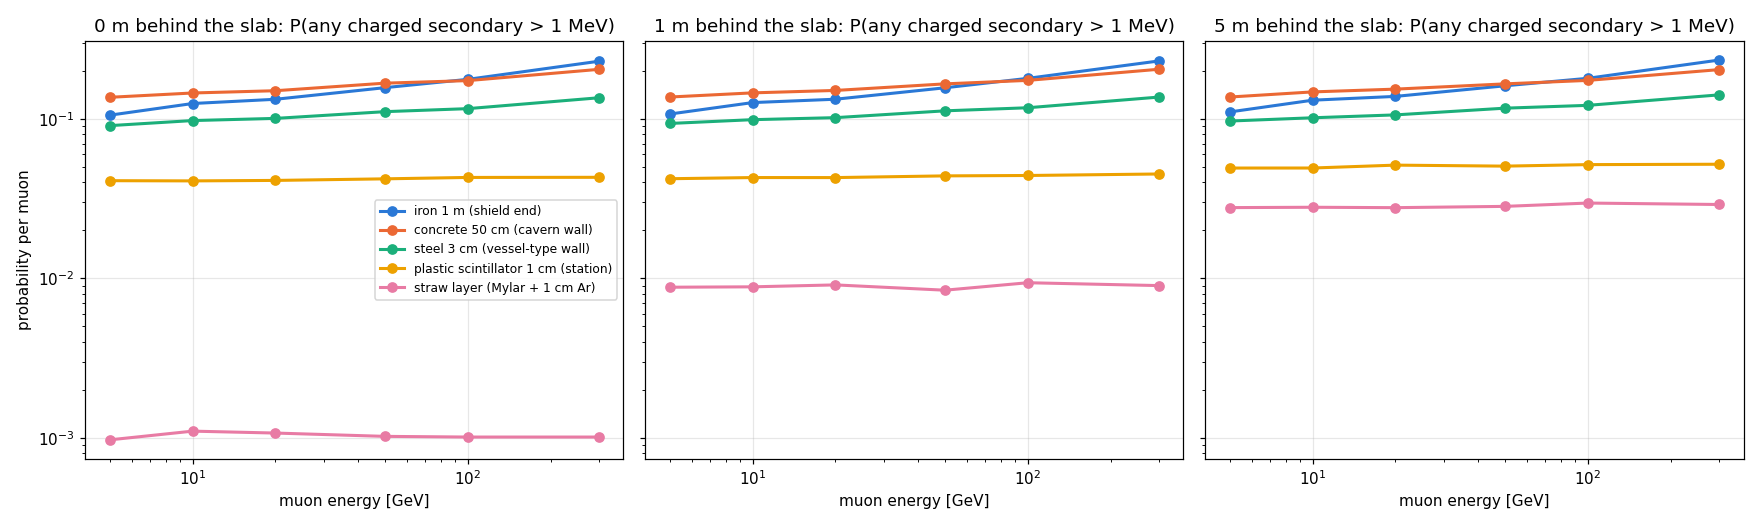
\includegraphics[width=\linewidth]{em_debris.png}
\caption{Probability of a charged secondary $>1$\,MeV behind an iron slab vs muon energy, at 0, 1 and 5\,m.
\src{lhcb_data .../results/em_debris/em_debris.png}}
\label{fig:debris}
\end{figure}

\section{Statistics and rare corners}

\begin{table}[h]
\centering\small
\caption{Is the statistics enough for a 15-year design number (\texttt{D6\_straw\_mod})?
\src{docs/STATUS.md (2026-11-10 day)}}
\begin{tabularx}{\linewidth}{@{}lX@{}}
\toprule
Source & State\\
\midrule
MS7 $K_L$ & lacking: 13 MC events selected, $\sim10^3$ per MC event $\Rightarrow$ $K_L$-enriched generation needed\\
vessel walls & lacking: 22 per MC event (cheap to fix)\\
helium & OK now ($\times20$ later)\\
neutrinos & sufficient\\
combinatorial & limited by the muon production (spills), not by transport; enough for the budget\\
cavern rock & $\sim7\times10^7$ per MC event: bound only by geometry\\
\bottomrule
\end{tabularx}
\end{table}

\begin{itemize}
\item Rare corners: step 1 = worst-case bounds from the stores per region of the interaction point
(\path{bin/coverage_bound.py}: MC count, selected / loose, $2.3\times$ mean-weight limit where none is selected).
First version, running. Later, where a corner is not bounded: splitting / weight windows in the shield transport,
forced neutral chains for rock and walls.
\item Storage: event stores 71\,GB, shell seeds 106\,GB, Nov-4 pool 145\,GB, dataset c 60\,GB, MS7 parents 10.8\,GB.
\item Tail extension (not run): \texttt{tail\_produce --mode complete} with a high threshold, $\sim$1--2 days + 1--5\,k
core-h; first decide which source tail is right (D5).
\end{itemize}

\section{Open issues and next steps}

From the issue review of 9 Nov 2026 (action list at the top of \path{ISSUES.txt}) plus D16 (10 Nov). Re-runs need
approval.

\begin{enumerate}
\item \textbf{D5} source tail: momentum convention ($\times0.905$) and tail angles ($\times0.56$) documented; enriched
sample kept as is, $+40\,\%$ source systematic on the SST1-selected rate. Decide which tail is right (also drives the
combinatorial $\times140$).
\item \textbf{D3} MS7 $K_L$ vs FairShip (priority A): chain default Geant4; small FairShip run on lxplus with our MS7
parents (like-for-like $K_L$ count at the iron exit and at SST1); D4: cut chords at the muon range.
\item \textbf{D16 / D9} V0: MS7 chain on the V0-stable library ($K_S$/$\Lambda$ $3\times$ low now); V0 tally in
\texttt{cpp/g4shield} (creator, vertex, fate: primary vs shower, total made); low-$W$ data check; add
$K_L\to\pi^+\pi^-$, $\gamma\gamma$ to the forced-decay table; multi-vertex rejection in the DIS$\times\mu$ pairs.
\item Code before the re-runs: D12 (\texttt{debris\_maps.py} $\to$ cross-check), C7 (forced $K_L$ decays in fastveto),
C1 (ghost hits), B4 (EventCalc re-import, benchmark set in the objective), A2 (bounce parameters free), D15 (import
retry + chunk check), D14 debris in time.
\item Neutrinos: 2026 flux adopted (done); D2 lateral-track veto with the signal loss.
\item Re-run batch in the FairShip layout at $4\times10^{13}$: stores / maps / inputs (C8, D8 Mylar), \texttt{run\_reco}
with both IP cuts, muon interactions with air margin, forced cavern Geant4, extra seeds (C5, A2), cross-run closure
(A1), EM debris (B2), DIS$\times\mu$ pairs (D9); B1 multiple-scattering check.
\item Statistics: $K_L$-enriched MS7 generation; more wall draws; coverage bounds (Sec.~8).
\item Tracking: ACTS (FairShip pixi 26.10, PR \#1545) resolution into \texttt{reco.measure}.
\item After the first optimum: FairShip validation of the optimised design (C3).
\end{enumerate}

\note{Questions to the detector colleagues: \path{docs/detector_questions.md}. Decided / closed: flat spill (A5),
cosmics ignored, $+x$ cavern wall not needed, parked shield muons accepted.}


\bibliographystyle{unsrt}
\bibliography{refs}
\end{document}
